%%% Template originaly created by Karol Kozioł (mail@karol-koziol.net) and modified for ShareLaTeX use

%%%------------------------------------------------------------------------------------------------%%%
%%%------------------------------------%%%     PREAMBLE     %%%------------------------------------%%%
%%%------------------------------------------------------------------------------------------------%%%

\documentclass[twoside=false,a4paper,11pt]{article}

\usepackage[T1]{fontenc}
\usepackage[utf8]{inputenc}
\usepackage{graphicx}
\usepackage{xcolor}

\usepackage{tgtermes}



\usepackage[
pdftitle={CPSC 471 Final Report},
pdfauthor={Timothy Mealey, University of Calgary},
colorlinks=true,linkcolor=blue,urlcolor=blue,citecolor=blue,bookmarks=true,
bookmarksopenlevel=2]{hyperref}
\usepackage{amsmath,amssymb,amsthm,textcomp}

\usepackage{enumitem}

\usepackage{multicol}
\usepackage{tikz}
\usetikzlibrary{shapes,positioning,calc}
\colorlet{lightgray}{gray!20}

\usepackage{geometry}
\geometry{total={210mm,297mm},
left=25mm,right=25mm,%
bindingoffset=0mm, top=20mm,bottom=20mm}

\linespread{1.3}

\newcommand{\linia}{\rule{\linewidth}{0.5pt}}

% custom theorems if needed
\newtheoremstyle{mytheor}
    {1ex}{1ex}{\normalfont}{0pt}{\scshape}{.}{1ex}
    {{\thmname{#1 }}{\thmnumber{#2}}{\thmnote{ (#3)}}}

\theoremstyle{mytheor}
\newtheorem{defi}{Definition}

% my own titles
\makeatletter
\renewcommand{\maketitle}{
\begin{center}
\vspace{2ex}
{\huge \textsc{\@title}}
\vspace{1ex}
\\
\linia\\
\@author \hfill \@date
\vspace{4ex}
\end{center}
}
\makeatother
%%%

% custom footers and headers
\usepackage{fancyhdr,lastpage}
\pagestyle{fancy}
\lhead{}
\chead{}
\rhead{}
\lfoot{Final Report}
\cfoot{}
\rfoot{Page \thepage\ /\ \pageref*{LastPage}}
\renewcommand{\headrulewidth}{0pt}
\renewcommand{\footrulewidth}{0pt}
%


%%%------------------------------------------------------------------------------------------------%%%
%%%------------------------------------%%%     DOCUMENT     %%%------------------------------------%%%
%%%------------------------------------------------------------------------------------------------%%%

\newcommand{\tuple}[2]{\{ #1 | #2 \}}
\newcommand{\domain}[2]{\{ (#1) | #2 \}}

\newcommand{\quantifier}[2]{(\ensuremath{#1}#2)}
\newcommand{\one}[1]{\quantifier{\exists}{#1}}
\newcommand{\all}[1]{\quantifier{\forall}{#1}}

\begin{document}

\title{CPSC 471 Final Report}
\author{Timothy Mealey, Ben Roberts, Cory Jensen, Scott Saunders}
\date{\today}
\maketitle

\section*{Abstract}

``An abstract of no more than 300 words.''

\section*{Introduction}

``Describe the problem or task your database was designed to address.
Describe (briefly) the system you have created to address the problem or task.''

\section*{Design}

\subsection*{Users}

``Discuss the different users of your system. Your discussion in this section should be considerably more detailed than what you described for the presentation - this section should describe a complete transaction collection and, consequently, provide a complete picture of the functionality offered by your system.''
%%Put in another file just to handle everything easily.


%\begin{enumerate}

%3 cases: browsing courses (Ie, not necessarily a student), building a schedule, creating an account,

%\item Browsing courses: \\

\subsection*{Browsing Courses}
%
%
%who:   Anyone interested in the courses offered by University of Calgary.
%what:  Course list.
%why:   Has detailed information, provided in a c
  %UofC calendar - no time information.
  %Ours: Has a powerful search, for dept, course number, and course name. %May not be entirely true.
%how:   One visits our page and searches for interesting topics by name, courses in particular, or just simply clicks things.
%
Anyone interested in the courses offered by the University of Calgary, would navigate to our website to evaluate potential classes. They would then search for preferred courses by topic, department, course numbers, or course names. Alternatively one could browse the convenient side-bar for a complete listing. As they select courses, the course info, availability and other information appears in the center of the screen.

\subsection*{Building Schedule}
%\item Building Schedule
%Who:   Anyone interested in attending the University of Calgary.
%what:  Course List and Schedule builder.
%When:  When the data is available!
%why:   Easily build schedules. Easy to enroll via these schedules.
%how:
%
Any Students or Perspective students getting organized for the upcoming semesters, would navigate to our website to construct a class schedule. Powered by the same technology of the dauwtrappen course list, one can find courses and add it to the schedule's selected courses. On this list the user is provided a listing of class times for each section of the class, which they can then select the times they want. If a mistake was made, simply clicking the thing again... Once the user has the schedule to their liking, there are course numbers provided such that the user will be able to use these numbers to enroll directly in those classes via the my.ucalgary.ca Enrollment: add


\subsection*{Login System}
%\item Login System
%Who:   Anyone interested in attending the University of Calgary.
%what:  An account for our system.
%why:   Used to self-organize courses, and curate your own schedules. //Not yet fully implemented.
%how:   Create an account, Verify Account, login!
%

Any new students, prospective students, or returning students, may use the login/account system to curate their own schedules, and checkup on their own interested courses. They would accomplish this by creating an account, (which adds them to the database), and verifying their email. From then on, they are free to login, and see any personalized data sets.
%\end{enumerate}


\subsubsection*{Log In}
\subsubsection*{Course Search}
\subsubsection*{Schedule Creator}

\subsection*{Entity Relationship Diagram}

\includegraphics[width=\textwidth]{ERDiagram.png}

``Any changes that were made since the presentation should be clearly indicated.''

\section*{Implementation}

\subsection*{Relational Schema Diagram}

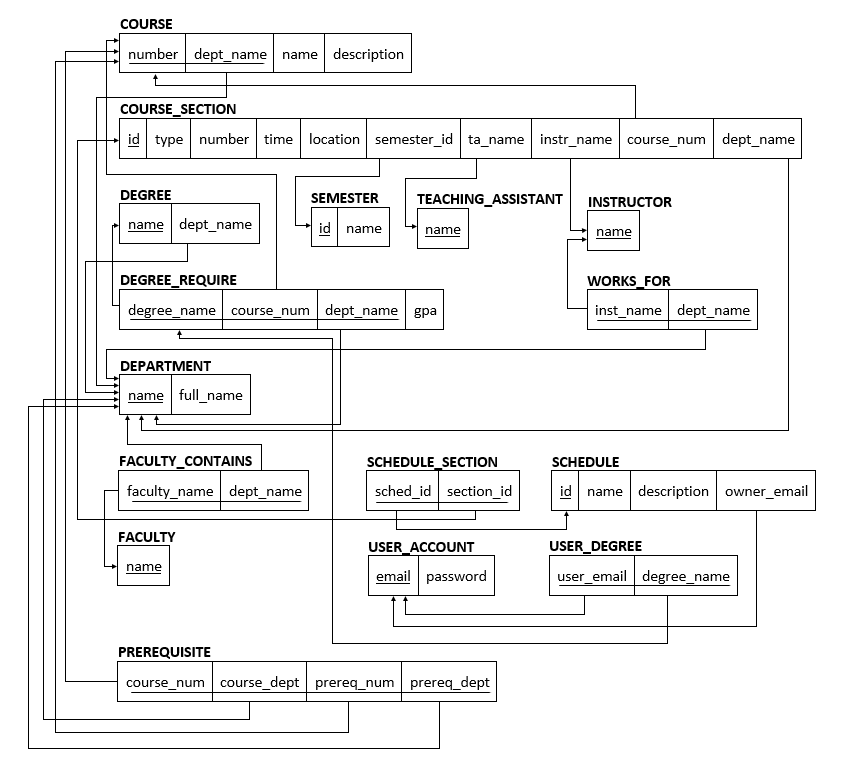
\includegraphics[width=\textwidth]{RelationalSchemaDiagram.png}

``Discuss any significant or unusual decisions made during this process.''

\subsection*{Database Management System}

``Describe the DBMS you selected for the implementation	of the project, and include the SQL statements for each of the transactions implemented. It is not necessary to discuss these transactions in relational algebra or calculus.''

\subsection*{User Interface}

``Present a brief description of your interface design, including several screenshots.''

\end{document}
